\section{Fundamentos Matematicos}
\label{sec:fundamentos}

En esta seccion se presentan las bases matematicas de las curvas de Bezier y de los dos metodos de evaluacion comparados en el estudio: la evaluacion directa mediante polinomios de Bernstein y el algoritmo de De Casteljau. Para cada metodo se describe su formulacion, su costo computacional y su comportamiento numerico, junto con sus ventajas y desventajas.

\subsection{Curvas de Bezier}
\label{subsec:fund_bezier}

Una curva de Bezier de grado $n$ queda definida por $n+1$ puntos de control $P_0, P_1, \dots, P_n$ en el plano. La curva comienza en $P_0$, termina en $P_n$ y los puntos intermedios actuan como atractores que dan forma al trazo, sin que la curva tenga que pasar por ellos \cite{farin2002}. El grado se obtiene directamente de la cantidad de puntos:
\begin{equation}
\label{eq:fund_grado}
n = (\text{cantidad de puntos de control}) - 1
\end{equation}

La curva se describe en forma parametrica mediante una funcion $C(t)$, donde el parametro $t$ recorre el intervalo $[0, 1]$. Como una computadora no puede evaluar infinitos valores de $t$, la curva se aproxima con $N$ muestras equiespaciadas:
\begin{equation}
\label{eq:fund_muestreo}
t_k = \frac{k}{N - 1}, \qquad k = 0, 1, \dots, N - 1
\end{equation}

Con esta eleccion la primera muestra corresponde a $t_0 = 0$ (punto $P_0$) y la ultima a $t_{N-1} = 1$ (punto $P_n$). Los puntos obtenidos se unen con segmentos de recta para dibujar la curva, sin recurrir a funciones graficas que generen curvas.

\subsection{Evaluacion mediante Polinomios de Bernstein}
\label{subsec:fund_bernstein}

La forma explicita de la curva de Bezier se expresa como una suma ponderada de los puntos de control, donde cada peso es un polinomio base de Bernstein \cite{farin2002,piegl1997}:
\begin{equation}
\label{eq:bernstein}
C(t) = \sum_{i=0}^{n} B_{i,n}(t)\, P_i, \qquad t \in [0, 1]
\end{equation}
\begin{equation}
\label{eq:fund_base}
B_{i,n}(t) = \binom{n}{i} (1 - t)^{n-i}\, t^{i}
\end{equation}

Cada componente de la curva se calcula por separado: $x(t) = \sum B_{i,n}(t)\, x_i$ e $y(t) = \sum B_{i,n}(t)\, y_i$. En la Figura~\ref{fig:fund_bases} se muestran las cuatro funciones base para el caso cubico ($n = 3$).

\begin{figure}[H]
\centering
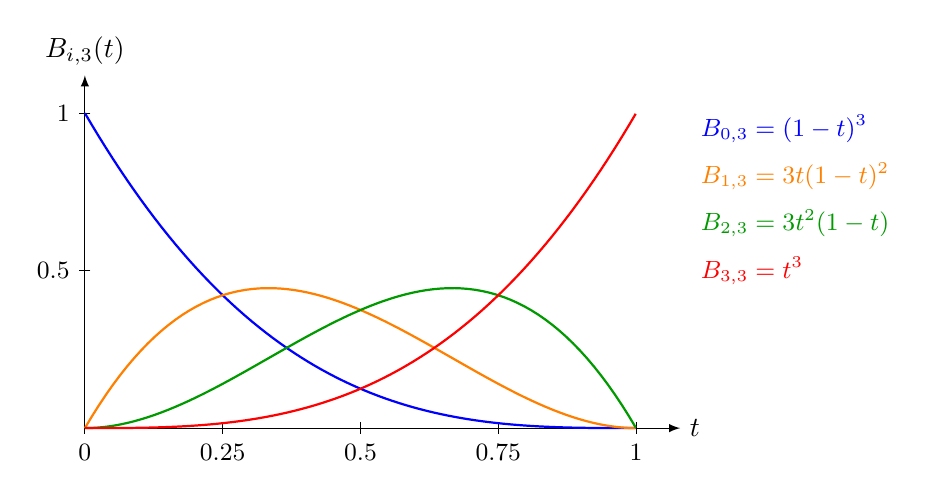
\begin{tikzpicture}[x=7cm, y=4cm]
  % Ejes
  \draw[-latex] (0,0) -- (1.08,0) node[right] {$t$};
  \draw[-latex] (0,0) -- (0,1.12) node[above] {$B_{i,3}(t)$};
  \foreach \xv in {0, 0.25, 0.5, 0.75, 1} {
    \draw (\xv,0.02) -- (\xv,-0.02) node[below] {\small $\xv$};
  }
  \foreach \yv in {0.5, 1} {
    \draw (0.01,\yv) -- (-0.01,\yv) node[left] {\small $\yv$};
  }
  % Funciones base de Bernstein para n = 3
  \draw[thick, blue, domain=0:1, samples=80] plot (\x, {(1-\x)^3});
  \draw[thick, orange, domain=0:1, samples=80] plot (\x, {3*\x*(1-\x)^2});
  \draw[thick, green!60!black, domain=0:1, samples=80] plot (\x, {3*\x^2*(1-\x)});
  \draw[thick, red, domain=0:1, samples=80] plot (\x, {\x^3});
  % Leyenda
  \node[blue, right] at (1.1,0.95) {\small $B_{0,3} = (1-t)^3$};
  \node[orange, right] at (1.1,0.80) {\small $B_{1,3} = 3t(1-t)^2$};
  \node[green!60!black, right] at (1.1,0.65) {\small $B_{2,3} = 3t^2(1-t)$};
  \node[red, right] at (1.1,0.50) {\small $B_{3,3} = t^3$};
\end{tikzpicture}
\caption{Polinomios base de Bernstein de grado 3 en el intervalo $[0, 1]$.}
\label{fig:fund_bases}
\end{figure}

Las bases de Bernstein cumplen propiedades que explican el comportamiento de la curva \cite{farin2002}:
\begin{itemize}
  \item \textbf{No negatividad:} $B_{i,n}(t) \ge 0$ para todo $t \in [0, 1]$.
  \item \textbf{Particion de la unidad:} $\sum_{i=0}^{n} B_{i,n}(t) = 1$, por lo que cada punto de la curva es un promedio ponderado de los puntos de control y la curva queda dentro de su envolvente convexa.
  \item \textbf{Interpolacion de extremos:} $C(0) = P_0$ y $C(1) = P_n$.
  \item \textbf{Simetria:} $B_{i,n}(t) = B_{n-i,n}(1 - t)$.
\end{itemize}

\subsubsection{Calculo de los coeficientes binomiales}

El coeficiente $\binom{n}{i}$ podria calcularse con factoriales, pero $n!$ crece tan rapido que desborda los tipos numericos aun para grados moderados (por ejemplo, $21!$ ya supera el maximo de un entero de 64 bits). Por ello se usa la relacion iterativa:
\begin{equation}
\label{eq:fund_binomial}
\binom{n}{0} = 1, \qquad \binom{n}{i} = \binom{n}{i-1} \cdot \frac{n - i + 1}{i}, \quad i = 1, \dots, n
\end{equation}

Los $n+1$ coeficientes dependen solo del grado y no del parametro $t$, por lo que se calculan una sola vez por curva, fuera del ciclo de muestras, con un costo de $\mathcal{O}(n)$.

\subsubsection{Convencion $0^0 = 1$}

En los extremos $t = 0$ y $t = 1$ aparecen expresiones de la forma $0^0$. Por ejemplo, en $t = 0$ el termino $i = 0$ contiene $t^0 = 0^0$. Para que se cumpla la interpolacion de extremos, se adopta la convencion $0^0 = 1$, de modo que $B_{0,n}(0) = 1$ y $B_{n,n}(1) = 1$. En la implementacion esta regla se aplica de forma explicita: si el exponente es cero, la potencia vale 1.

\subsection{Algoritmo de De Casteljau}
\label{subsec:fund_casteljau}

El algoritmo de De Casteljau obtiene el mismo punto $C(t)$ sin usar los polinomios de Bernstein, mediante interpolaciones lineales sucesivas entre pares de puntos consecutivos \cite{farin2002,piegl1997}. Se parte de los puntos de control como nivel inicial, $P_i^{(0)} = P_i$, y se aplica la recurrencia:
\begin{equation}
\label{eq:casteljau}
P_i^{(r)} = (1 - t)\, P_i^{(r-1)} + t\, P_{i+1}^{(r-1)}, \qquad r = 1, \dots, n, \quad i = 0, \dots, n - r
\end{equation}

Cada nivel $r$ tiene un punto menos que el anterior, y al llegar al nivel $r = n$ queda un unico punto, que es el punto de la curva:
\begin{equation}
\label{eq:fund_casteljau_resultado}
C(t) = P_0^{(n)}
\end{equation}

Para el caso cubico ($n = 3$) los niveles forman el siguiente esquema triangular, donde cada punto se obtiene de los dos puntos que tiene encima:
\begin{equation}
\label{eq:fund_triangulo}
\begin{array}{ccccccc}
P_0^{(0)} &  & P_1^{(0)} &  & P_2^{(0)} &  & P_3^{(0)} \\
 & P_0^{(1)} &  & P_1^{(1)} &  & P_2^{(1)} &  \\
 &  & P_0^{(2)} &  & P_1^{(2)} &  &  \\
 & & & P_0^{(3)} = C(t) & & &
\end{array}
\end{equation}

Geometricamente, cada nivel divide los segmentos del nivel anterior en la proporcion $t : (1 - t)$. Estas construcciones intermedias son las interpolaciones que la aplicacion dibuja en color verde. En la Seccion~\ref{sec:validacion} se desarrolla un ejemplo numerico completo con $t = 0.5$.

\subsection{Analisis de Complejidad}
\label{subsec:fund_complejidad}

Para comparar ambos metodos se cuenta el numero de operaciones necesarias para una curva de grado $n$ evaluada en $N$ muestras.

\textbf{Bernstein.} En cada muestra se suman $n + 1$ terminos (Ecuacion~\ref{eq:bernstein}). Cada termino requiere dos potencias, $(1-t)^{n-i}$ y $t^{i}$, y algunas multiplicaciones de costo constante. Como los coeficientes binomiales ya estan precalculados, el costo por muestra es $\mathcal{O}(n)$ y el costo total es:
\begin{equation}
\label{eq:fund_costo_bernstein}
T_{B}(n, N) = \underbrace{\mathcal{O}(n)}_{\text{coeficientes}} + \underbrace{N \cdot \mathcal{O}(n)}_{\text{muestras}} = \mathcal{O}(N \cdot n)
\end{equation}

\textbf{De Casteljau.} En cada muestra, el nivel $r$ realiza $n - r + 1$ interpolaciones (Ecuacion~\ref{eq:casteljau}). Sumando todos los niveles:
\begin{equation}
\label{eq:fund_operaciones_casteljau}
\sum_{r=1}^{n} (n - r + 1) = n + (n - 1) + \dots + 1 = \frac{n(n+1)}{2}
\end{equation}
\begin{equation}
\label{eq:fund_costo_casteljau}
T_{DC}(n, N) = N \cdot \frac{n(n+1)}{2} = \mathcal{O}(N \cdot n^2)
\end{equation}

En ambos metodos el costo crece de forma lineal con la cantidad de muestras $N$. La diferencia esta en el grado: al duplicar $n$, el tiempo de Bernstein se duplica, mientras que el de De Casteljau se multiplica aproximadamente por cuatro. El Cuadro~\ref{tab:fund_complejidad} resume estos resultados.

\begin{table}[H]
\centering
\caption{Complejidad teorica de ambos metodos para una curva de grado $n$ evaluada en $N$ muestras.}
\label{tab:fund_complejidad}
\begin{tabular}{lcc}
\toprule
\textbf{Aspecto} & \textbf{Bernstein} & \textbf{De Casteljau} \\
\midrule
Preparacion por curva & $\mathcal{O}(n)$ (coeficientes) & No requiere \\
Operaciones por muestra & $n + 1$ terminos & $n(n+1)/2$ interpolaciones \\
Costo por muestra & $\mathcal{O}(n)$ & $\mathcal{O}(n^2)$ \\
Costo total & $\mathcal{O}(N \cdot n)$ & $\mathcal{O}(N \cdot n^2)$ \\
Memoria adicional & $\mathcal{O}(n)$ (coeficientes) & $\mathcal{O}(n)$ (copia de puntos) \\
Uso de potencias & Si, $2(n+1)$ por muestra & No \\
\bottomrule
\end{tabular}
\end{table}

La notacion asintotica no considera las constantes ocultas. Cada llamada a una funcion de potencia es mas costosa que una multiplicacion simple, por lo que en grados bajos De Casteljau puede competir con Bernstein aunque su orden sea mayor. Los tiempos reales se analizan en las Secciones~\ref{sec:experimentacion} y \ref{sec:comparacion}.

\subsection{Estabilidad Numerica}
\label{subsec:fund_estabilidad}

Ambos metodos producen la misma curva en aritmetica exacta, pero en una computadora se trabaja con numeros de punto flotante de doble precision (IEEE 754 de 64 bits), que tienen alrededor de 15 a 16 cifras decimales significativas \cite{ieee754}. Cada operacion introduce un pequeno error de redondeo, y la forma en que estos errores se acumulan depende del metodo.

\textbf{De Casteljau} solo realiza combinaciones convexas: en la Ecuacion~\ref{eq:casteljau} los pesos $(1 - t)$ y $t$ estan entre 0 y 1 y suman 1. Por eso cada nuevo punto queda entre los dos anteriores y los errores no se amplifican de un nivel a otro. Esta propiedad hace que el algoritmo sea reconocido como numericamente estable \cite{farouki1987}.

\textbf{Bernstein} combina numeros de magnitudes muy distintas. Para grados altos los coeficientes binomiales crecen mucho; por ejemplo, $\binom{100}{50} \approx 1.01 \times 10^{29}$. Al mismo tiempo, las potencias $(1-t)^{n-i}$ y $t^{i}$ se vuelven muy pequenas. El producto de un numero muy grande por uno muy pequeno, junto con el error propio de la funcion de potencia, puede producir perdida de cifras significativas. En consecuencia, se espera que Bernstein se aleje mas de la curva exacta a medida que aumenta el grado. Esta hipotesis se verifica experimentalmente en la Seccion~\ref{sec:comparacion}.

\subsection{Ventajas y Desventajas}
\label{subsec:fund_ventajas}

El Cuadro~\ref{tab:fund_ventajas} resume las caracteristicas de cada metodo segun el analisis anterior.

\begin{table}[H]
\centering
\caption{Ventajas y desventajas de los metodos de evaluacion de curvas de Bezier.}
\label{tab:fund_ventajas}
\begin{tabular}{p{2.2cm} p{6cm} p{6cm}}
\toprule
\textbf{Metodo} & \textbf{Ventajas} & \textbf{Desventajas} \\
\midrule
Bernstein &
Costo $\mathcal{O}(n)$ por muestra. Formula directa: cada punto se calcula de forma independiente. Permite precalcular los coeficientes. &
Usa potencias y coeficientes binomiales grandes. Pierde precision en grados altos. No entrega la construccion geometrica intermedia. \\
\midrule
De Casteljau &
Numericamente estable por usar combinaciones convexas. Solo usa sumas y multiplicaciones. Sus niveles intermedios permiten visualizar la construccion y subdividir la curva. &
Costo $\mathcal{O}(n^2)$ por muestra. Su tiempo crece mas rapido con el grado. Requiere copiar los puntos en cada muestra. \\
\bottomrule
\end{tabular}
\end{table}

% RESUMEN: Esta seccion (02_fundamentos.tex) define las curvas de Bezier, el muestreo
% t_k = k/(N-1), la forma de Bernstein (eq:bernstein, eq:fund_base, eq:fund_binomial,
% convencion 0^0 = 1), la recurrencia de De Casteljau (eq:casteljau), la complejidad
% O(N n) vs O(N n^2) (tab:fund_complejidad), la estabilidad numerica y una tabla de
% ventajas y desventajas (tab:fund_ventajas). Incluye la figura TikZ fig:fund_bases (no
% requiere captura). Etiquetas que otros referencian: sec:fundamentos, eq:bernstein,
% eq:casteljau. Usa \ref{sec:validacion}, \ref{sec:experimentacion} y \ref{sec:comparacion}.
% Citas: farin2002, piegl1997, farouki1987, ieee754 (las mismas de Andres).
% El equipo debe verificar que esas cuatro claves existan en referencias.bib.
